\documentclass[tikz,border=8pt]{standalone}
\usepackage{tikz}
\usepackage{fontawesome5}
\usepackage{amsmath,amssymb}
\usetikzlibrary{arrows.meta,positioning,fit,backgrounds,calc,shadows,shapes.geometric}

% Lavender & Slate Color Palette
\definecolor{lavenderDark}{RGB}{15, 44, 89}
\definecolor{lavenderDeep}{RGB}{10, 28, 58}
\definecolor{lavenderMedium}{RGB}{29, 78, 158}
\definecolor{lavenderLight}{RGB}{240, 246, 255}
\definecolor{lavenderBorder}{RGB}{180, 205, 237}
\definecolor{lavenderAccent}{RGB}{2, 132, 199}
\definecolor{prismNavy}{RGB}{15, 44, 89}
\definecolor{prismBlue}{RGB}{29, 78, 158}
\definecolor{prismTeal}{RGB}{13, 148, 136}
\definecolor{prismMint}{RGB}{236, 253, 245}
\definecolor{prismGold}{RGB}{217, 119, 6}
\definecolor{prismDark}{RGB}{15, 23, 42}
\definecolor{prismLight}{RGB}{248, 250, 252}

\begin{document}
% End-to-End System Flow for CiviQ Indian Legal RAG System
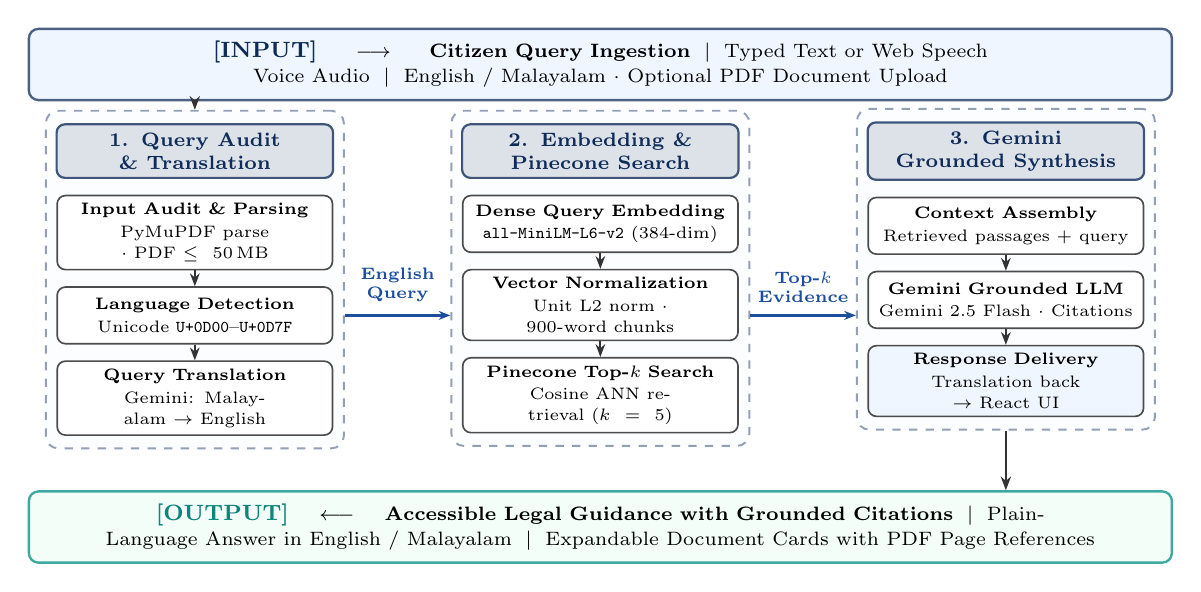
\begin{tikzpicture}[
    x=1cm, y=1cm,
    font=\sffamily,
    inout/.style={
        rectangle, rounded corners=3.5pt, line width=0.85pt,
        inner sep=4.5pt, align=center,
        font=\fontsize{7.5}{9.0}\selectfont
    },
    hdrbox/.style={
        rectangle, draw=lavenderDark!80, line width=0.80pt, fill=lavenderDark!14,
        rounded corners=3pt, inner sep=3.0pt, align=center,
        text width=3.30cm,
        font=\fontsize{7.2}{8.5}\selectfont\bfseries\color{lavenderDark}
    },
    stepbox/.style={
        rectangle, draw=black!70, line width=0.60pt, fill=white,
        rounded corners=3pt, inner sep=2.8pt, align=center,
        text width=3.30cm, minimum height=0.72cm,
        font=\fontsize{6.5}{7.6}\selectfont
    },
    stagebox/.style={
        rectangle, draw=lavenderDark!45, dashed, rounded corners=4.5pt, line width=0.70pt,
        fill=lavenderLight!25, inner xsep=3.5pt, inner ysep=4.5pt
    },
    flowarr/.style={
        -{Stealth[scale=0.75]}, line width=0.70pt, draw=black!80
    },
    transarr/.style={
        -{Stealth[length=4.2pt, width=3.2pt]}, line width=1.0pt, draw=lavenderMedium
    }
]

    % 1. TOP: INPUT BAR (width = 14.2cm)
    \node [inout, fill=lavenderLight, draw=lavenderDark!75, text width=14.2cm] (input_node) at (0, 3.60) {
        \textbf{\fontsize{7.8}{9.0}\selectfont\color{lavenderDark}[INPUT]} $\;\longrightarrow\;$
        \textbf{Citizen Query Ingestion}\; $\vert$\;
        {\fontsize{6.6}{7.8}\selectfont Typed Text or Web Speech Voice Audio}\; $\vert$\;
        {\fontsize{6.6}{7.8}\selectfont English / Malayalam $\cdot$ Optional PDF Document Upload}
    };

    % 2. MIDDLE: 3-STAGE HORIZONTAL PIPELINE
    % Spaced at x = -5.15, x = 0.00, x = +5.15 with text width = 3.30cm

    % --- STAGE 1: INGESTION & TRANSLATION (x = -5.15) ---
    \node [hdrbox] (h1) at (-5.15, 2.50) {1. Query Audit \& Translation};
    
    \node [stepbox, below=0.20cm of h1] (s1_1) {
        \textbf{Input Audit \& Parsing}\\[0.08em]
        {\fontsize{6.0}{7.0}\selectfont PyMuPDF parse $\cdot$ PDF $\le 50$\,MB}
    };
    \node [stepbox, below=0.20cm of s1_1] (s1_2) {
        \textbf{Language Detection}\\[0.08em]
        {\fontsize{6.0}{7.0}\selectfont Unicode \texttt{U+0D00}--\texttt{U+0D7F}}
    };
    \node [stepbox, below=0.20cm of s1_2] (s1_3) {
        \textbf{Query Translation}\\[0.08em]
        {\fontsize{6.0}{7.0}\selectfont Gemini: Malayalam $\to$ English}
    };

    \draw [flowarr] (s1_1) -- (s1_2);
    \draw [flowarr] (s1_2) -- (s1_3);

    \begin{scope}[on background layer]
    \node [stagebox, fit=(h1) (s1_3)] (stage1) {};
    \end{scope}

    % --- STAGE 2: EMBEDDING & RETRIEVAL (x = 0.00) ---
    \node [hdrbox] (h2) at (0.00, 2.50) {2. Embedding \& Pinecone Search};
    
    \node [stepbox, below=0.20cm of h2] (s2_1) {
        \textbf{Dense Query Embedding}\\[0.08em]
        {\fontsize{6.0}{7.0}\selectfont \texttt{all-MiniLM-L6-v2} (384-dim)}
    };
    \node [stepbox, below=0.20cm of s2_1] (s2_2) {
        \textbf{Vector Normalization}\\[0.08em]
        {\fontsize{6.0}{7.0}\selectfont Unit L2 norm $\cdot$ 900-word chunks}
    };
    \node [stepbox, below=0.20cm of s2_2] (s2_3) {
        \textbf{Pinecone Top-$k$ Search}\\[0.08em]
        {\fontsize{6.0}{7.0}\selectfont Cosine ANN retrieval ($k=5$)}
    };

    \draw [flowarr] (s2_1) -- (s2_2);
    \draw [flowarr] (s2_2) -- (s2_3);

    \begin{scope}[on background layer]
    \node [stagebox, fit=(h2) (s2_3)] (stage2) {};
    \end{scope}

    % --- STAGE 3: GENERATION & CITATIONS (x = +5.15) ---
    \node [hdrbox] (h3) at (5.15, 2.50) {3. Gemini Grounded Synthesis};
    
    \node [stepbox, below=0.20cm of h3] (s3_1) {
        \textbf{Context Assembly}\\[0.08em]
        {\fontsize{6.0}{7.0}\selectfont Retrieved passages + query}
    };
    \node [stepbox, below=0.20cm of s3_1] (s3_2) {
        \textbf{Gemini Grounded LLM}\\[0.08em]
        {\fontsize{6.0}{7.0}\selectfont Gemini 2.5 Flash $\cdot$ Citations}
    };
    \node [stepbox, below=0.20cm of s3_2, fill=lavenderLight] (s3_3) {
        \textbf{Response Delivery}\\[0.08em]
        {\fontsize{6.0}{7.0}\selectfont Translation back $\to$ React UI}
    };

    \draw [flowarr] (s3_1) -- (s3_2);
    \draw [flowarr] (s3_2) -- (s3_3);

    \begin{scope}[on background layer]
    \node [stagebox, fit=(h3) (s3_3)] (stage3) {};
    \end{scope}

    % Common elevation coordinate for perfectly horizontal inter-stage arrows
    \path let \p1 = (s1_2.center) in coordinate (transY) at (0, \y1);

    % Horizontal Transition Arrows in the Gap (2-line compact label, zero collision)
    \draw [transarr] (stage1.east |- transY) -- node[above=1pt, align=center, font=\fontsize{5.8}{6.8}\selectfont\bfseries\color{lavenderMedium}]{English\\Query} (stage2.west |- transY);
    \draw [transarr] (stage2.east |- transY) -- node[above=1pt, align=center, font=\fontsize{5.8}{6.8}\selectfont\bfseries\color{lavenderMedium}]{Top-$k$\\Evidence} (stage3.west |- transY);

    % Connect Top Input to Stage 1
    \draw [flowarr, line width=0.80pt] (input_node.south -| stage1.north) -- (stage1.north);

    % 3. BOTTOM: OUTPUT BAR (Positioned below stage boxes with 0.55cm clean margin)
    \node [inout, fill=prismMint!65, draw=prismTeal!80, text width=14.2cm, below=0.55cm of stage2] (output_node) {
        \textbf{\fontsize{7.8}{9.0}\selectfont\color{prismTeal!90!black}[OUTPUT]} $\;\longleftarrow\;$
        \textbf{Accessible Legal Guidance with Grounded Citations}\; $\vert$\;
        {\fontsize{6.6}{7.8}\selectfont Plain-Language Answer in English / Malayalam}\; $\vert$\;
        {\fontsize{6.6}{7.8}\selectfont Expandable Document Cards with PDF Page References}
    };

    % Connect Stage 3 to Output Bar
    \draw [flowarr, line width=0.80pt] (stage3.south) -- (output_node.north -| stage3.south);

\end{tikzpicture}
\end{document}
